\documentclass[a0paper,portrait]{baposter}

\usepackage[utf8]{inputenc}
\usepackage{relsize}	       % For \smaller
\usepackage{url}			       % For \url
\usepackage{multicol}        % Multi Columns
\renewcommand{\familydefault}{\sfdefault}
%\usepackage{helvet}

%%%%%%%%%%%%%%%%%%%%%%%%%%%%%%%%%%%%%%%%%%%%%%%%%%%%%%%%%%%%%%%%%%%%%%%%%%%%%%%%
%%% Utility functions %%%%%%%%%%%%%%%%%%%%%%%%%%%%%%%%%%%%%%%%%%%%%%%%%%%%%%%%%%
%%%%%%%%%%%%%%%%%%%%%%%%%%%%%%%%%%%%%%%%%%%%%%%%%%%%%%%%%%%%%%%%%%%%%%%%%%%%%%%%

%%% Save space in lists. Use this after the opening of the list %%%%%%%%%%%%%%%%
\renewcommand{\vec}[1]{\bm{#1}}
\newcommand{\vnabla}{\vec{\nabla}}

\renewcommand{\d}[1]{\text{d} #1}
\newcommand{\dxx}{\,\text{d}\vec{x}}
\newcommand{\dx}{\,\text{d}x}

\newcommand{\diff}[2]{\frac{\text{d}#1}{\text{d}#2}}
\newcommand{\idiff}[2]{\text{d}#1 / \text{d}#2}
\newcommand{\pdiff}[2]{\frac{\partial #1}{\partial #2}}
\newcommand{\pdifff}[2]{\frac{\partial^2 #1}{\partial #2^2}}
\newcommand{\ipdiff}[2]{\partial #1 / \partial #2}
\newcommand{\vdiff}[2]{\frac{\delta #1}{\delta #2}}
\newcommand{\ivdiff}[2]{\delta #1 / \delta #2}

%%%%%%%%%%%%%%%%%%%%%%%%%%%%%%%%%%%%%%%%%%%%%%%%%%%%%%%%%%%%%%%%%%%%%%%%%%%%%%%
%%% Document Start %%%%%%%%%%%%%%%%%%%%%%%%%%%%%%%%%%%%%%%%%%%%%%%%%%%%%%%%%%%%
%%%%%%%%%%%%%%%%%%%%%%%%%%%%%%%%%%%%%%%%%%%%%%%%%%%%%%%%%%%%%%%%%%%%%%%%%%%%%%%

\begin{document}
\typeout{Poster rendering started}

%%% General Poster Settings %%%%%%%%%%%%%%%%%%%%%%%%%%%%%%%%%%%%%%%%%%%%%%%%%%%
%%%%%% Eye Catcher, Title, Authors and University Images %%%%%%%%%%%%%%%%%%%%%%
\begin{poster}{
  columns=3,
	grid=false,
	borderColor=red,
	headerColorOne=red,
	headerColorTwo=red,
	headerFontColor=white,
  headerheight=10em,
	boxColorOne=white,
  boxpadding=1em,
	headershape=rounded,
	headerfont=\Large\textsf,
	textborder=rounded,
	background=shadetb,
  bgColorOne=red!10,
  bgColorTwo=red!30,
	headerborder=open,
  boxshade=plain,
  eyecatcher=false
}
%%% Eye Cacther %%%%%%%%%%%%%%%%%%%%%%%%%%%%%%%%%%%%%%%%%%%%%%%%%%%%%%%%%%%%%%%
{
}
%%% Title %%%%%%%%%%%%%%%%%%%%%%%%%%%%%%%%%%%%%%%%%%%%%%%%%%%%%%%%%%%%%%%%%%%%%
{\Huge \textcolor{red}{International HPC Certification Program}}
%%% Authors %%%%%%%%%%%%%%%%%%%%%%%%%%%%%%%%%%%%%%%%%%%%%%%%%%%%%%%%%%%%%%%%%%%
{
  \vspace{1em}
  Julian Kunkel$^1$, Kai Himstedt$^2$, Weronika Filinger$^3$, Jean-Thomas Acquaviva$^4$, William Jalby$^5$, Lev Lafayette$^6$

  \vspace*{-0.5em}
  {\small $^1$:University of Reading, $^2$:Universität Hamburg, $^3$:EPCC, $^4$: DDN, $^5$: Université de Versailles Saint-Quentin, $^6$: University of Melbourne}\\

  \vspace*{-0.5em}

  \huge \url{https://www.hpc-certification.org/}
}
%%% Logo %%%%%%%%%%%%%%%%%%%%%%%%%%%%%%%%%%%%%%%%%%%%%%%%%%%%%%%%%%%%%%%%%%%%%%
{%\begin{minipage}{20.0em}
    %\includegraphics[height=5em]{logo-uni}
 % \end{minipage}
}

%%% Abstract %%%%%%%%%%%%%%%%%%%%%%%%%%%%%%%%%%%%%%%%%%%%%%%%%%%%%%%%%%%%%%%%%%
\headerbox{Abstract}{name=abstract,column=0,row=0,span=2}{
\begin{multicols}{2}
\textit{%
The HPC community has always considered the training of new and existing HPC practitioners to be of high importance to its growth. The significance of training will increase even further in the era of Exascale when HPC encompasses even more scientific disciplines. This diversification of HPC practitioners challenges the traditional training approaches, which are not able to satisfy the specific needs of users, often coming from non-traditionally HPC disciplines and only interested in learning a particular set of skills. HPC centres are struggling to identify and overcome the gaps in users’ knowledge. How should we support prospective and existing users who are not aware of their own knowledge gaps?
We are working towards the establishment of an International HPC Certification program that would clearly categorize, define and examine them similarly to a school curriculum.
Ultimately, we aim for the certificates to be recognized and respected by the HPC community and industry.
}
\end{multicols}
}


\headerbox{Competences and Skills}{name=box12,column=0,below=abstract, span=2}{
Various competencies are necessary to efficiently use HPC resources.
A skill is a meaningful competence that comes with a \textbf{clear definition} of knowledge/practical ability, \textbf{levels of knowledge}, \textbf{relations to other skills}.
An excerpt of the first levels of the skill-tree developed by the \textit{PeCoH project} is used as starting point:

\medskip

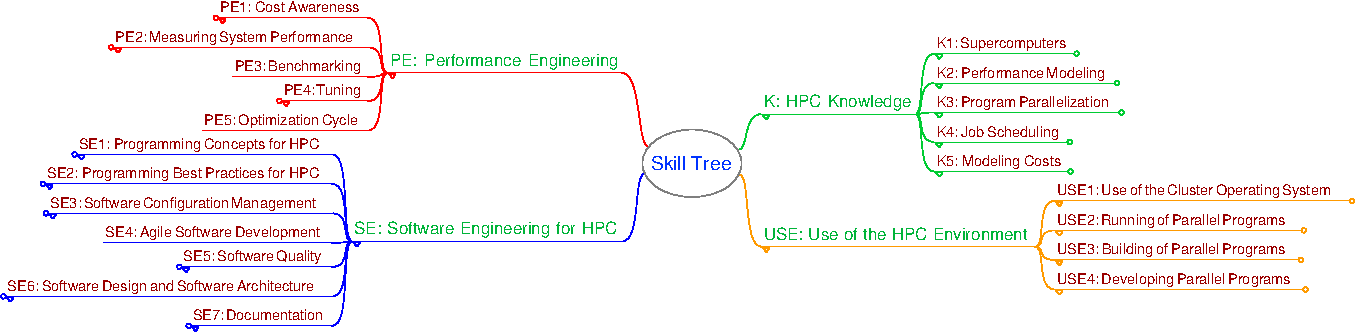
\includegraphics[width=1\textwidth]{1-crop.pdf}
%\includegraphics[width=\textwidth, height=6cm]{skill-tree-auto-generated_180412a.png}
% \includegraphics[width=\textwidth, trim=2cm 28cm 2cm 0cm, clip]{skill-tree-auto-generated_180412a.pdf}

\medskip


The skill-handbook is available in various representations on the webpage and as XML on our GitHub organization: \url{https://github.com/hpc-certification-forum}.
}

\headerbox{Benefits}{name=benefits,column=0,below=box12}{
  %\begin{columns}
   % \column{0.5\textwidth}
    \textbf{HPC practitioners}
    \vspace*{-0.5em}
      \begin{itemize}
        \setlength\itemsep{-0.3em}
      \item Increase motivation to participate
      \item (Certificates are recognized in CV)
      \item Validate knowledge via tests
      \item Browse of relevant competences
      \item Identify recommended and required skills
      \item Compare teaching offers across sites
  	  \end{itemize}

	%\column{0.5\textwidth}
    \textbf{Data centers}
    \vspace*{-0.5em}
      \begin{itemize}
        \setlength\itemsep{-0.3em}

      \item Increase sharing of teaching materials
      \item Documentation of taught skills simplified
      \item Identify missing teaching activities
      \item Tailor skill-tree specifically to users
      \item Correlate lack of skills with efficient use
  	  \end{itemize}
  %\end{columns}%
}

\headerbox{Status}{name=status,column=0,below=benefits, above=bottom}{

PeCoH delivered a concept paper, skill-tree, and a Javascript visualization.
Technically, skills are stored in an XML document and can be processed via XSLT into various representations.
The Javascripts can be re-used and configured by anyone -- e.g., for linking teaching material.

\medskip

In progress: forming a governance body.

\smallskip

\textbf{Responsibilities of the governance body}:
\vspace*{-0.5em}
  \begin{itemize}
  \setlength\itemsep{-0.3em}
  \item Steering the program
  \item Curating the curriculum
  	%\vspace*{-0.5em}
  	%\begin{itemize}
%    	\setlength\itemsep{0em}
 %   	\item Curating the skill-handbook
  %      \item Defining certificates on skill sets
   % \end{itemize}
  \item Performing the exams
  	%\vspace*{-0.5em}
  	%\begin{itemize}
    %\setlength\itemsep{0em}
    %\item First approach: Online
    %\end{itemize}
  \end{itemize}
  \vspace*{-0.5em}
  It is \textbf{not} its duty to interfere with content! We aim to preserve the teaching ecosystem.

}


\headerbox{Get Involved!}{name=box2,column=1,below=box12,above=bottom}{
This is an independent community-wide effort.

\bigskip

\textbf{Who can join?}

%\begin{itemize}
%\item
Anyone (person or organization) experienced or interested in HPC teaching and training.
%\end{itemize}

\bigskip

\textbf{What can we contribute?}

There are various levels of contribution
\vspace*{-0.4em}
\begin{itemize}
\setlength\itemsep{-0.3em}
\item developing skill-tree scope and content
\item becoming ambassador for the program
\item steering of the governance body
\end{itemize}
\vspace*{-0.4em}

Simply visit our website \url{hpc-certification.org} and join the mailing lists!

\bigskip

\textbf{What does it cost to join?}

It is free to join for everyone!
However, for \textbf{full members} (with voting rights), we expect a minimum contribution to the overall program.
Note that anyone joining will be listed on the public webpage!

\medskip
\textbf{Meetings:}

A general assembly of members will occur at least twice a year -- presumably during ISC and SC.
On a monthly basis, the program chair organizes a conference call, that shall be attended by  the executive board but open to members.

\medskip
\textbf{Providing teaching material:}

Since the certification program itself curates the curriculum but does not provide teaching material, anyone is welcome to provide teaching material -- we can help with checking and will support branding!
}

\headerbox{The PeCoH Project}{name=pecoh,column=2}{
	The Performance Conscious HPC (PeCoH) project* aimed to create a lightweight HPC certification program. During the first year, it became apparent to broaden the scope and form an independent governance entity to sustain the effort and gain acceptance. Project information:
    \begin{itemize}%[noitemsep,nolistsep]
    \item DFG funded (runtime: 2017-2019)
    \item Partners
    	\vspace*{-0.5em}
    	\begin{itemize}
        \item Universität Hamburg (UHAM)
        \item Regional computing center UHAM
        \item Computer Center of Hamburg University of Technology (TUHH RZ)
        \end{itemize}
    \item Methods:
    	\vspace*{-0.5em}
    	\begin{itemize}
        	\item Competence management
            \item Cost-Awareness
            \item Success stories
            \item Explore benefit of new concepts
		\end{itemize}
    \end{itemize}
	{\tiny *:\url{https://wr.informatik.uni-hamburg.de/research/projects/pecoh/} }
}



\headerbox{Governance Rules}{name=governance,column=2,below=pecoh}{
We are in the process to establish rules with the members of the forum.
Envisioned executive roles for the board are:
\begin{itemize}
\setlength\itemsep{-0.3em}
\item Program chair (PC)
	\vspace*{-0.5em}
	\begin{itemize}
    \setlength\itemsep{-0.3em}
    \item Chairs the overall executive board
    \item Chairs meetings and conf. calls
    \end{itemize}
\item Curriculum chair (CC)
	\vspace*{-0.5em}
	\begin{itemize}
    \setlength\itemsep{-0.3em}
    \item Decides new curriculum releases
    \item Merges changes suggested by TC
    \end{itemize}
\item Topic chairs (TC)
	\vspace*{-0.5em}
	\begin{itemize}
    \setlength\itemsep{-0.3em}
    \item Curate skills of a subtree (e.g., XXX)
    \item Funnels change requests of members
    \end{itemize}
\item Examination chair (EC)
	\vspace*{-0.5em}
	\begin{itemize}
    \setlength\itemsep{-0.3em}
    \item Manages examination handling
    \end{itemize}
\item Publicity chair (PRC)
	\vspace*{-0.5em}
	\begin{itemize}
    \setlength\itemsep{-0.3em}
    \item Develops and implements PR strategy
    \end{itemize}
\end{itemize}

Everyone can offer or be recommended to fill any role.
Full members have voting rights; the vote with majority wins.

%\begin{itemize}
%\item Change management to the skills
%\item Definition of certificates
%\item Voting right
%\end{itemize}
}

\headerbox{Next steps}{name=next,column=2,below=governance}{
A first meeting takes place during ISC-HPC to establish initial governance rules, and define next steps. Everyone is welcome to attend.

\textbf{When}: Wed. 27. Jun. 2018 12:45 – 13:30 (bring your lunch) \\
\textbf{Where}: Exhibition hall, Lunch area, table closest to booth N-230 (project posters)


%The meeting takes place on \textbf{TODO fill final slot here}.
}

\headerbox{Acknowledgements}{name=box32,column=2,below=next,above=bottom}{
\scriptsize
The PeCoH project is supported by the German Research Foundation (DFG) under grants LU 1353/12-1, OL 241/2-1, and RI 1068/7-1.
}

\end{poster}
\end{document}
